\chapter{Methodology}\label{ch:methodology}

\section{Proposed System}

To solve the issues outlined in Chapter~\ref*{ch:lit_review}, in Thesis A, the following system was proposed.
Using a Microsoft Kinect v2 depth sensor, user's gestures can be detected and processed on an Ubuntu machine.
Utilising Robot Operating System (ROS) 2, once the gestures are processed, signals can be sent over the ROS network to control devices throughout the home.
Finally, a TypeScript (TS) frontend would be developed to enable users to customise their home to make the system adaptable to user needs.
This led to the initial simplified technology stack as shown in Figure~\ref{fig:simple_tech_stack}.

\begin{figure}[!htb]
    \caption{Simplified Technology Stack}
    \centering
    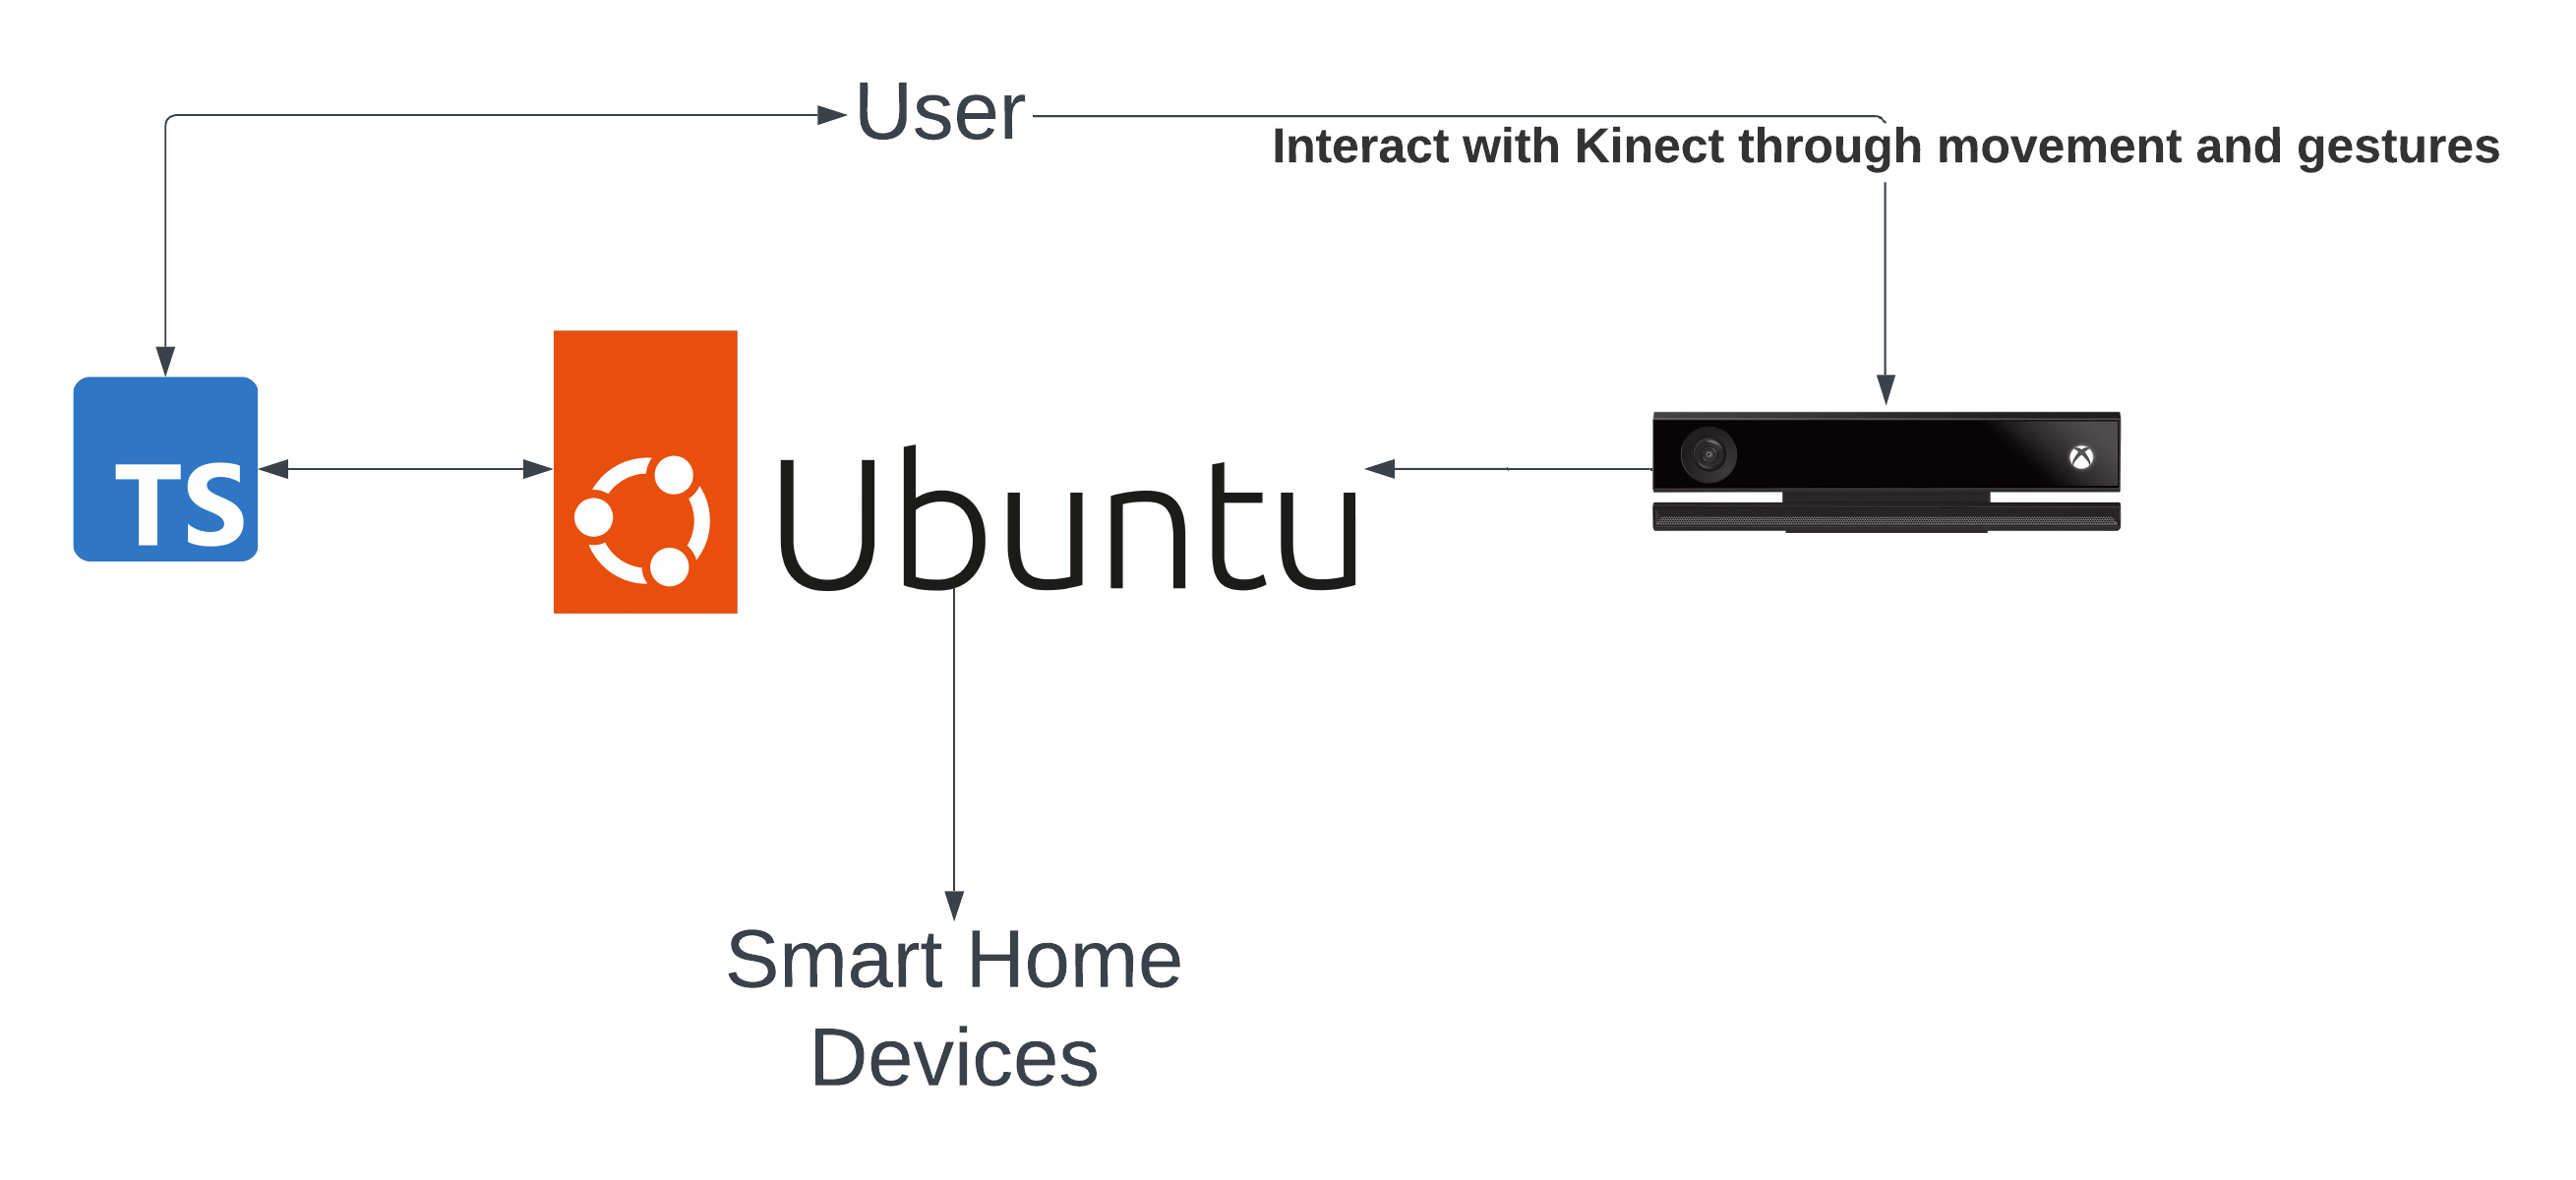
\includegraphics[width=0.88\textwidth]{Simplified Tech Stack.png}
    \label{fig:simple_tech_stack}
\end{figure}

\subsection{Technology Stack}
\subsubsection{Thesis A}
Throughout the development of this system, the technology stack gradually changed over time in order to accommodate growing goals and to overcome challenges.
In Thesis A, there were many challenges in getting the Kinect camera to communicate with ROS 2.
A very specific environment setup is required in order for these systems to function together reliably as shown in Figure~\ref{fig:tech_stack_thesis_a}.

\subsubsection{Thesis B}
Following this, during the complete development of the system in Thesis B, the technology stack was modified slightly in order to accomodate a more robust and customisable system for managing smart devices in the home as in Figure~\ref{fig:tech_stack_thesis_b}.
Using the open source home automation platform Home Assistant allows for far more versatility in automation abilities, choices for devices and provides it's own user interface, eliminating the need for a separate custom TS frontend.

\subsubsection{Thesis C}
During Thesis C, one of the stretch goals that was set, implementing voice commands and multi-modal device control, was developed.
This, again, made some minor changes to the technology stack, incorporating a new TS frontend for users to define their own custom voice commands, and a Vosk speech recognition model integrated as a node on the ROS network.
The final technology stack for this thesis as it is currently implemented is as shown in Figure~\ref{fig:tech_stack_thesis_c}

\begin{figure}[H]
    \caption{Thesis A Proposed Technology Stack}
    \makebox[\textwidth][c]{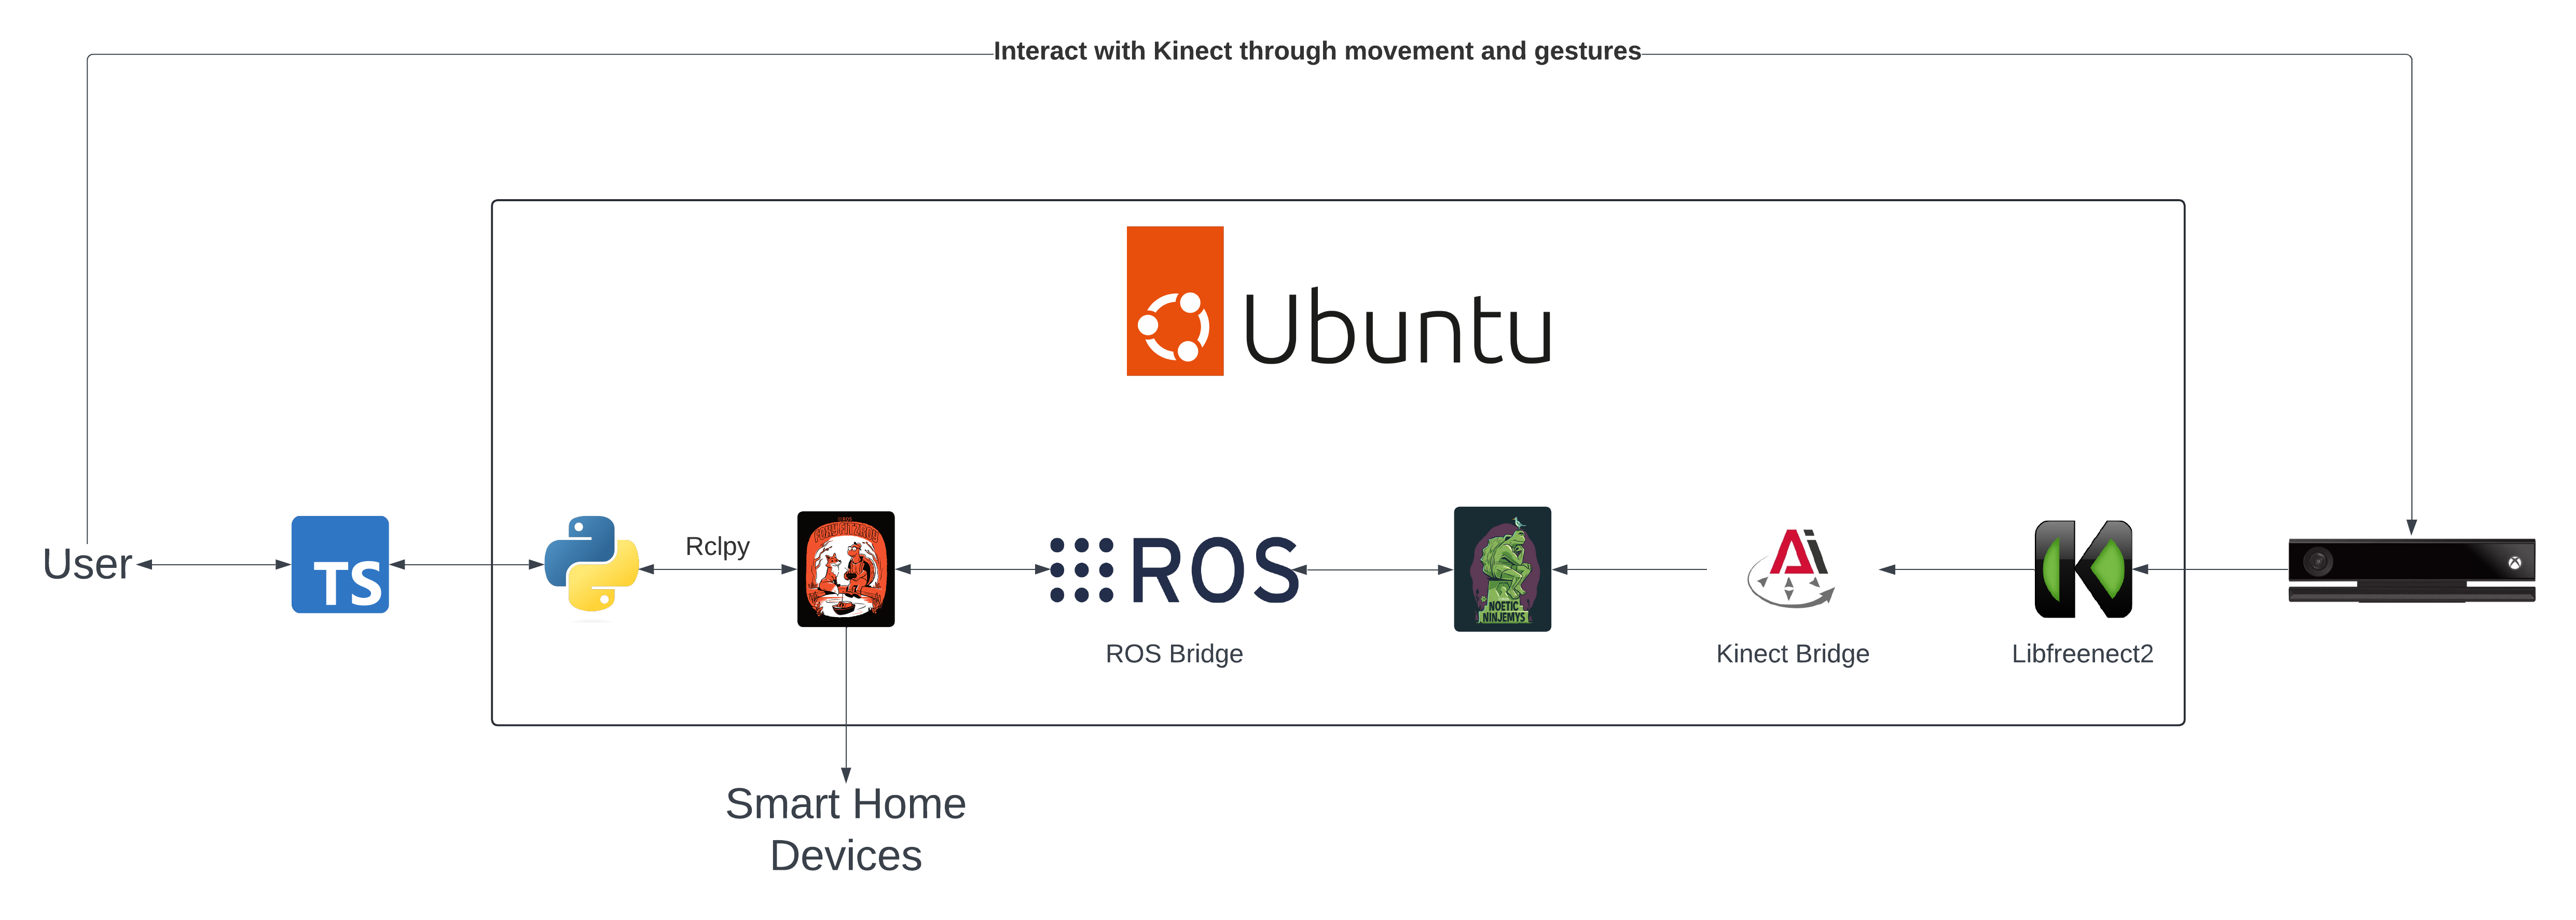
\includegraphics[width=\textheight,angle=90]{Tech Stack Thesis A.png}}
    \label{fig:tech_stack_thesis_a}
\end{figure}

\begin{figure}[H]
    \caption{Thesis B Implemented Technology Stack}
    \makebox[\textwidth][c]{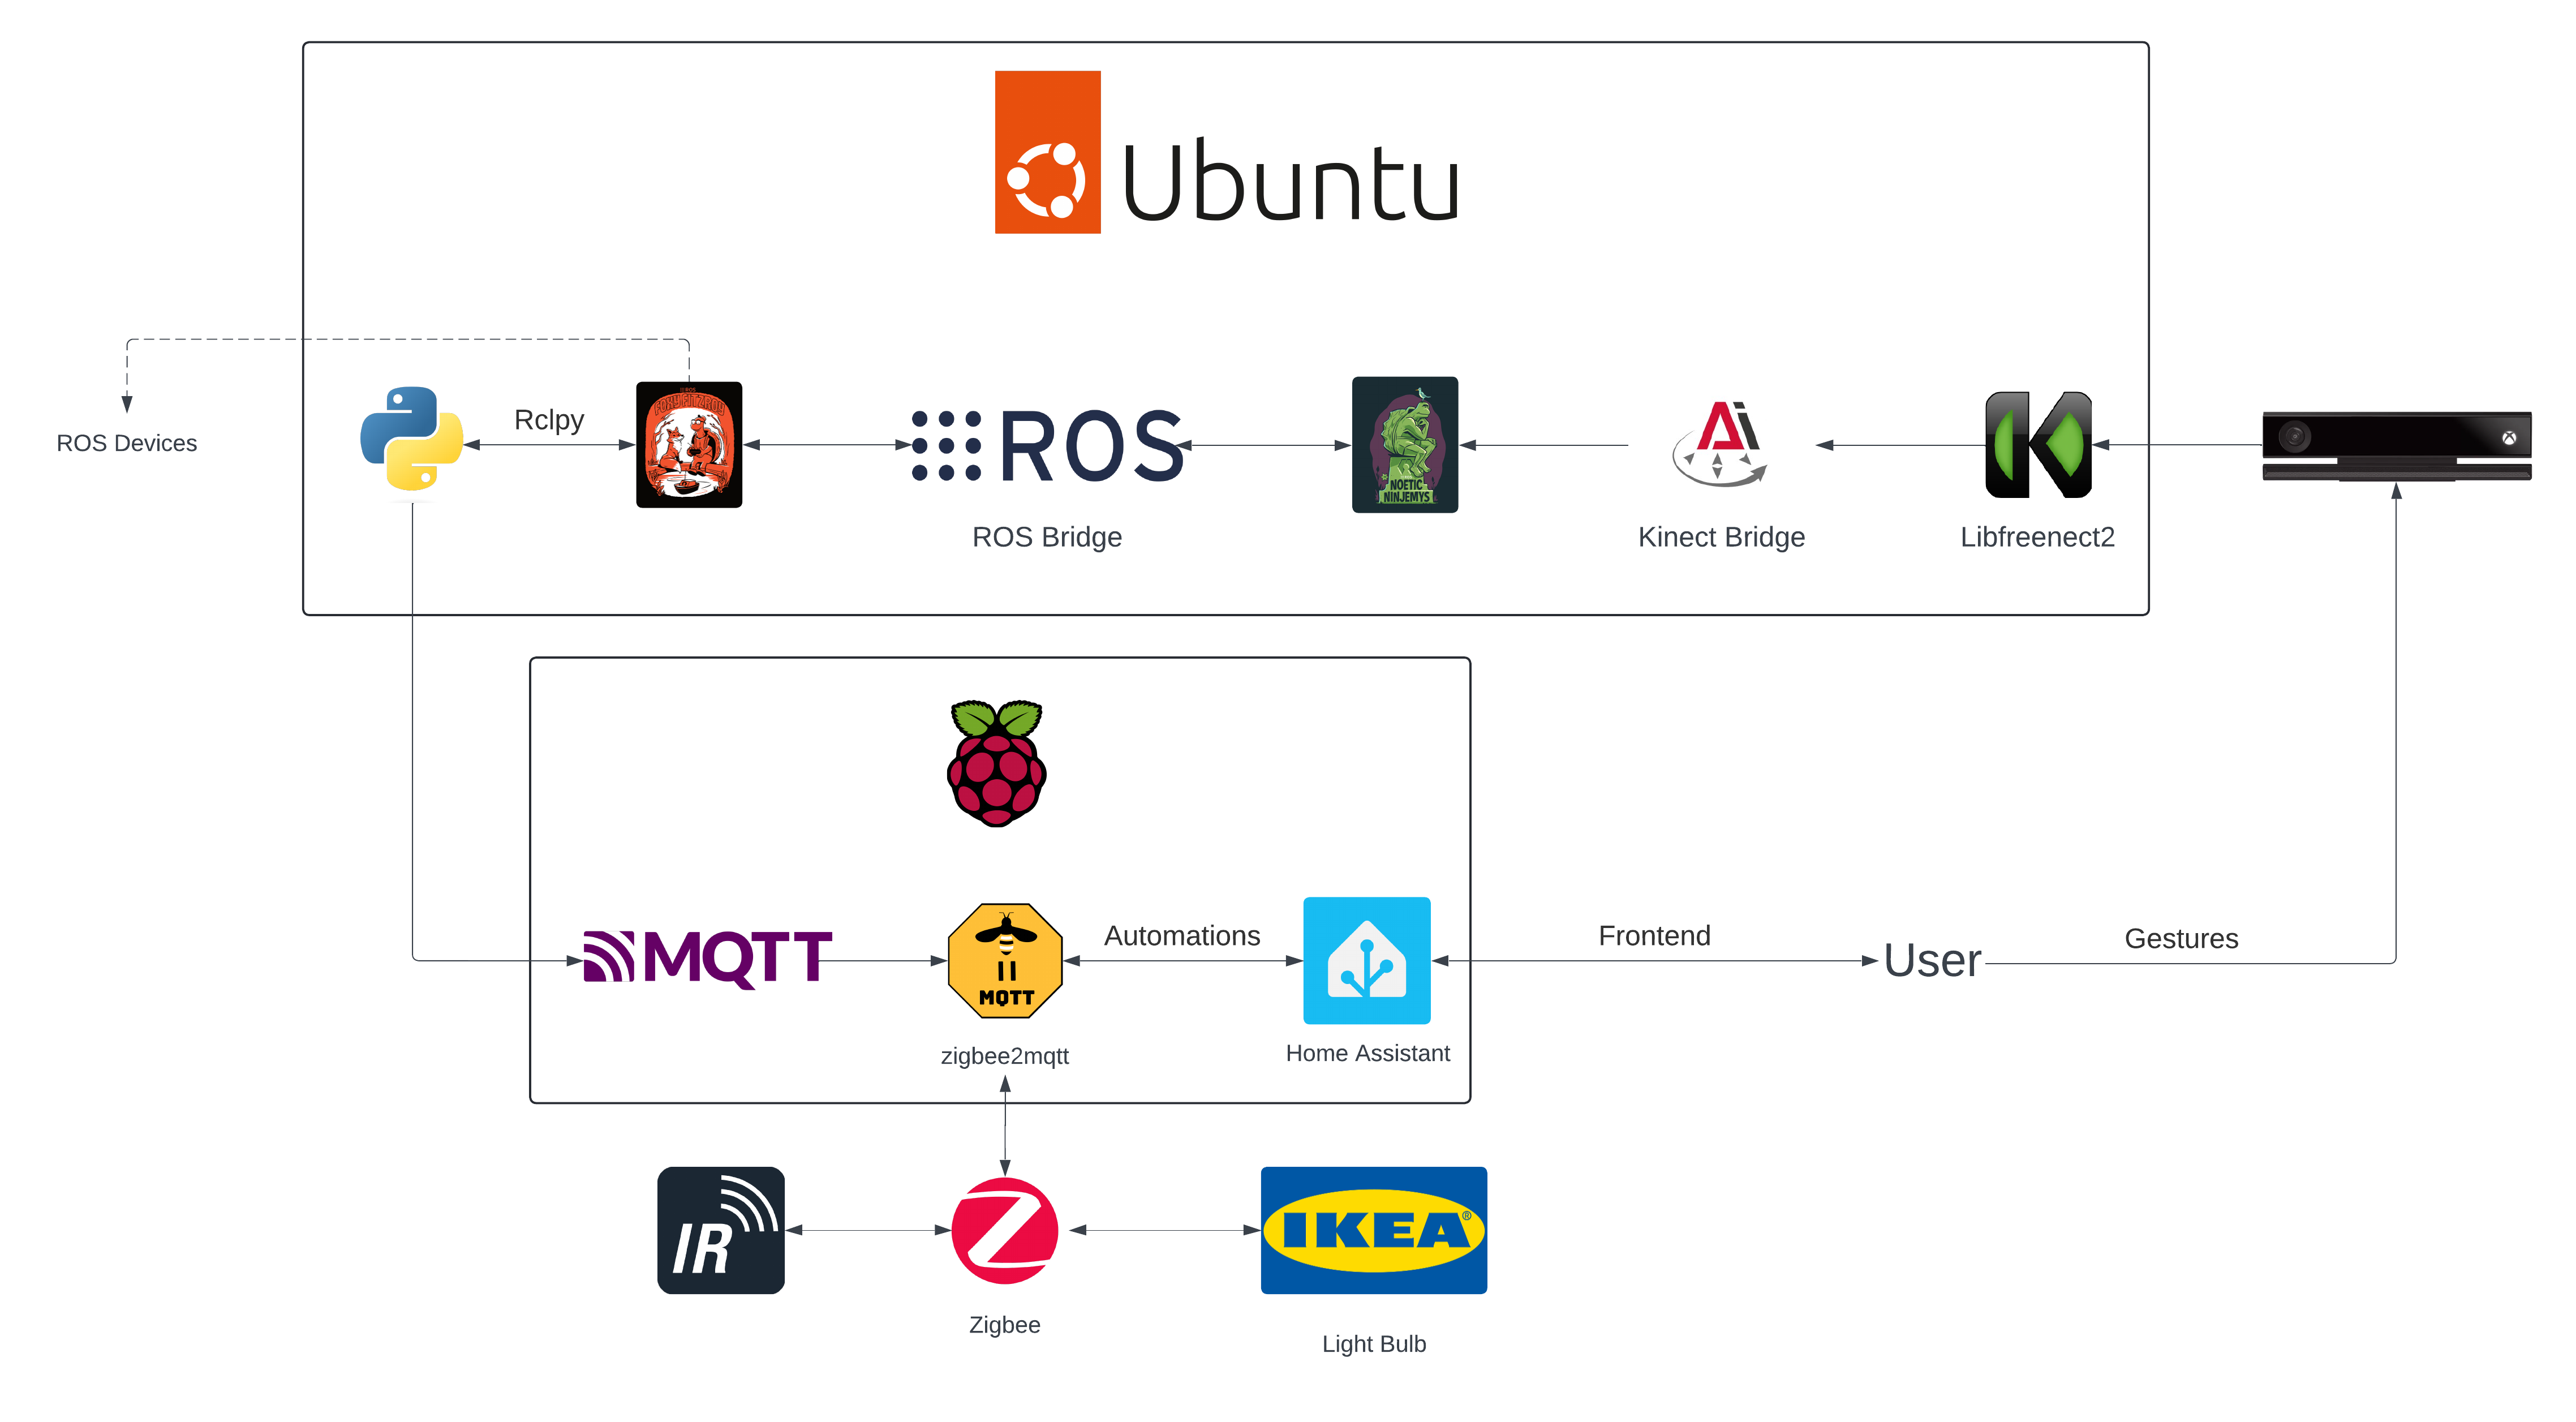
\includegraphics[width=\textheight,angle=-90]{Tech Stack Thesis B.png}}
    \label{fig:tech_stack_thesis_b}
\end{figure}

\begin{figure}[H]
    \caption{Thesis C Final Technology Stack}
    \makebox[\textwidth][c]{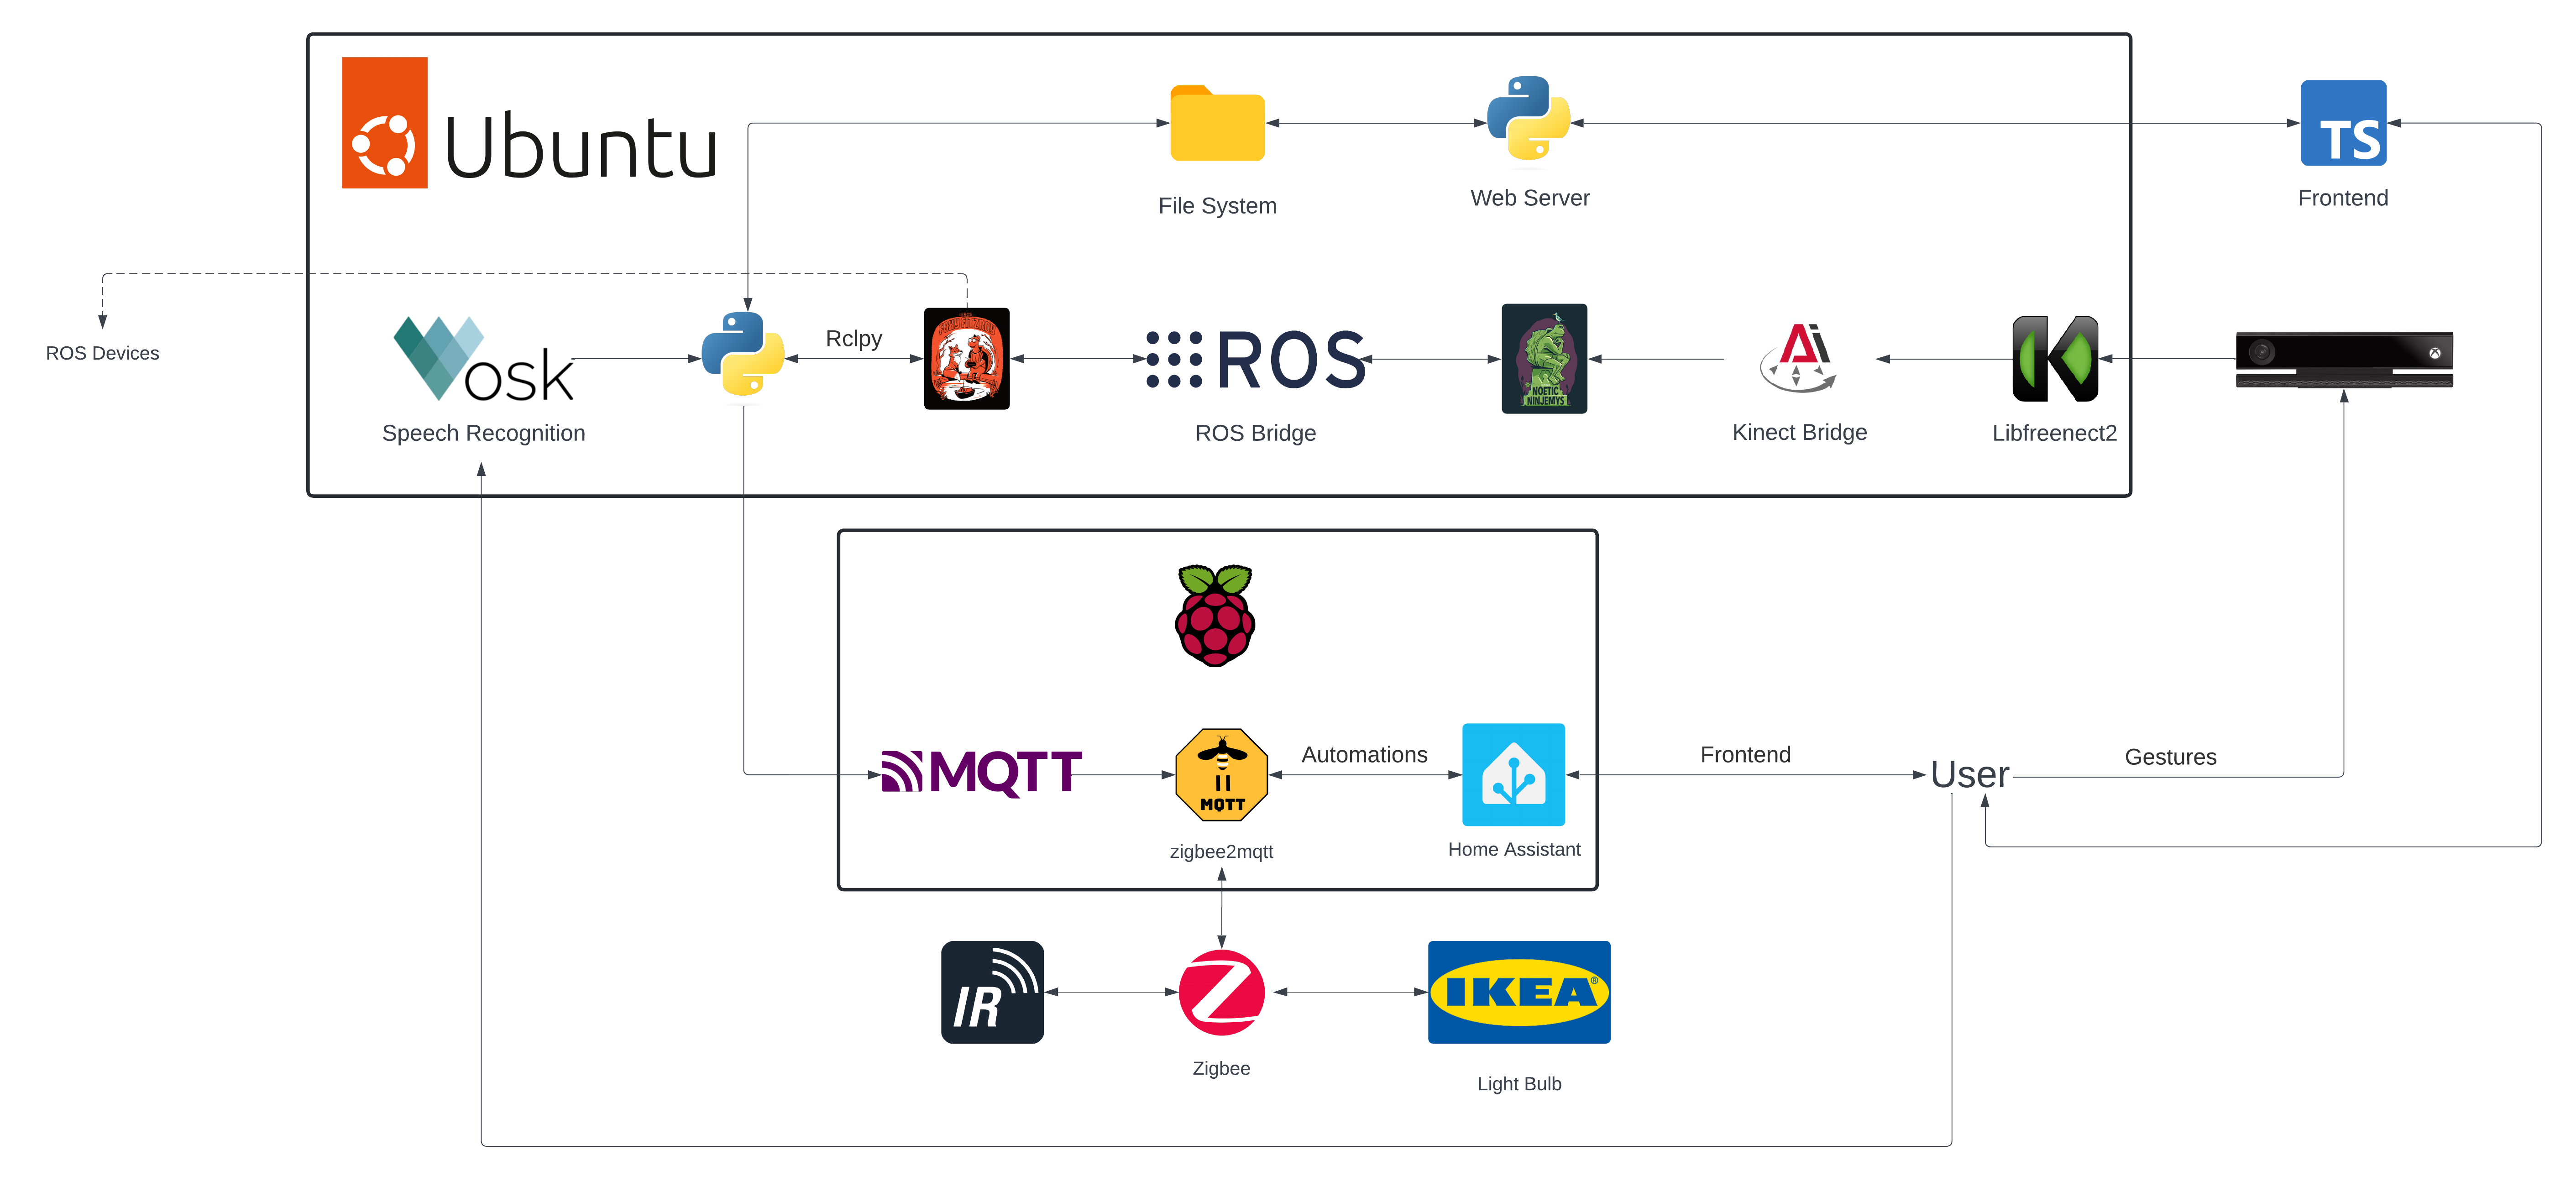
\includegraphics[width=\textheight,angle=90]{Tech Stack Thesis C.png}}
    \label{fig:tech_stack_thesis_c}
\end{figure}

\section{Hardware Components}
The hardware components used in the development of this system include the following:
\begin{itemize}
    \item Dell XPS15 9510 Laptop
    \item Microsoft Kinect v2
    \item Raspberry Pi 3
    \item Sonoff Zigbee 3.0 USB Dongle Plus
    \item Ikea Trådfri Zigbee Bulbs
    \item Zigbee IR Emitter
\end{itemize}

The selection of the Dell XSP15 Laptop was due to its immediate availability as it was already owned.
This is a powerful laptop with a discrete graphics card and was always sure to be capable of running the software required.
However, a laptop of this calibre is not completely necessary and most modern hardware should be sufficient.

The Microsoft Kinect v2 was also selected due to it being readily available.
This, however, is a necessary piece of equipment for this system as it is currently designed.
In theory, other depth cameras could be suitable for alternative deployments but this would require significant work to modify the existing environment setup and potentially large portions of the codebase.

The Raspberry Pi 3, was selected for multiple reasons.
Home Assistant is relatively lightweight so the choice of hardware was not limited by processing power, therefore a miniature computer such as a Raspberry Pi was appealling due to it's low cost, small footprint and ease of use with Home Assistant.
The Pi 3 specifically was chosen as it was available on-hand, though other single-board computers capable of running Home Assistant would also be fitting choices.

\begin{figure}[!htb]
    \caption{Home Assistant Interface}
    \makebox[\textwidth][c]{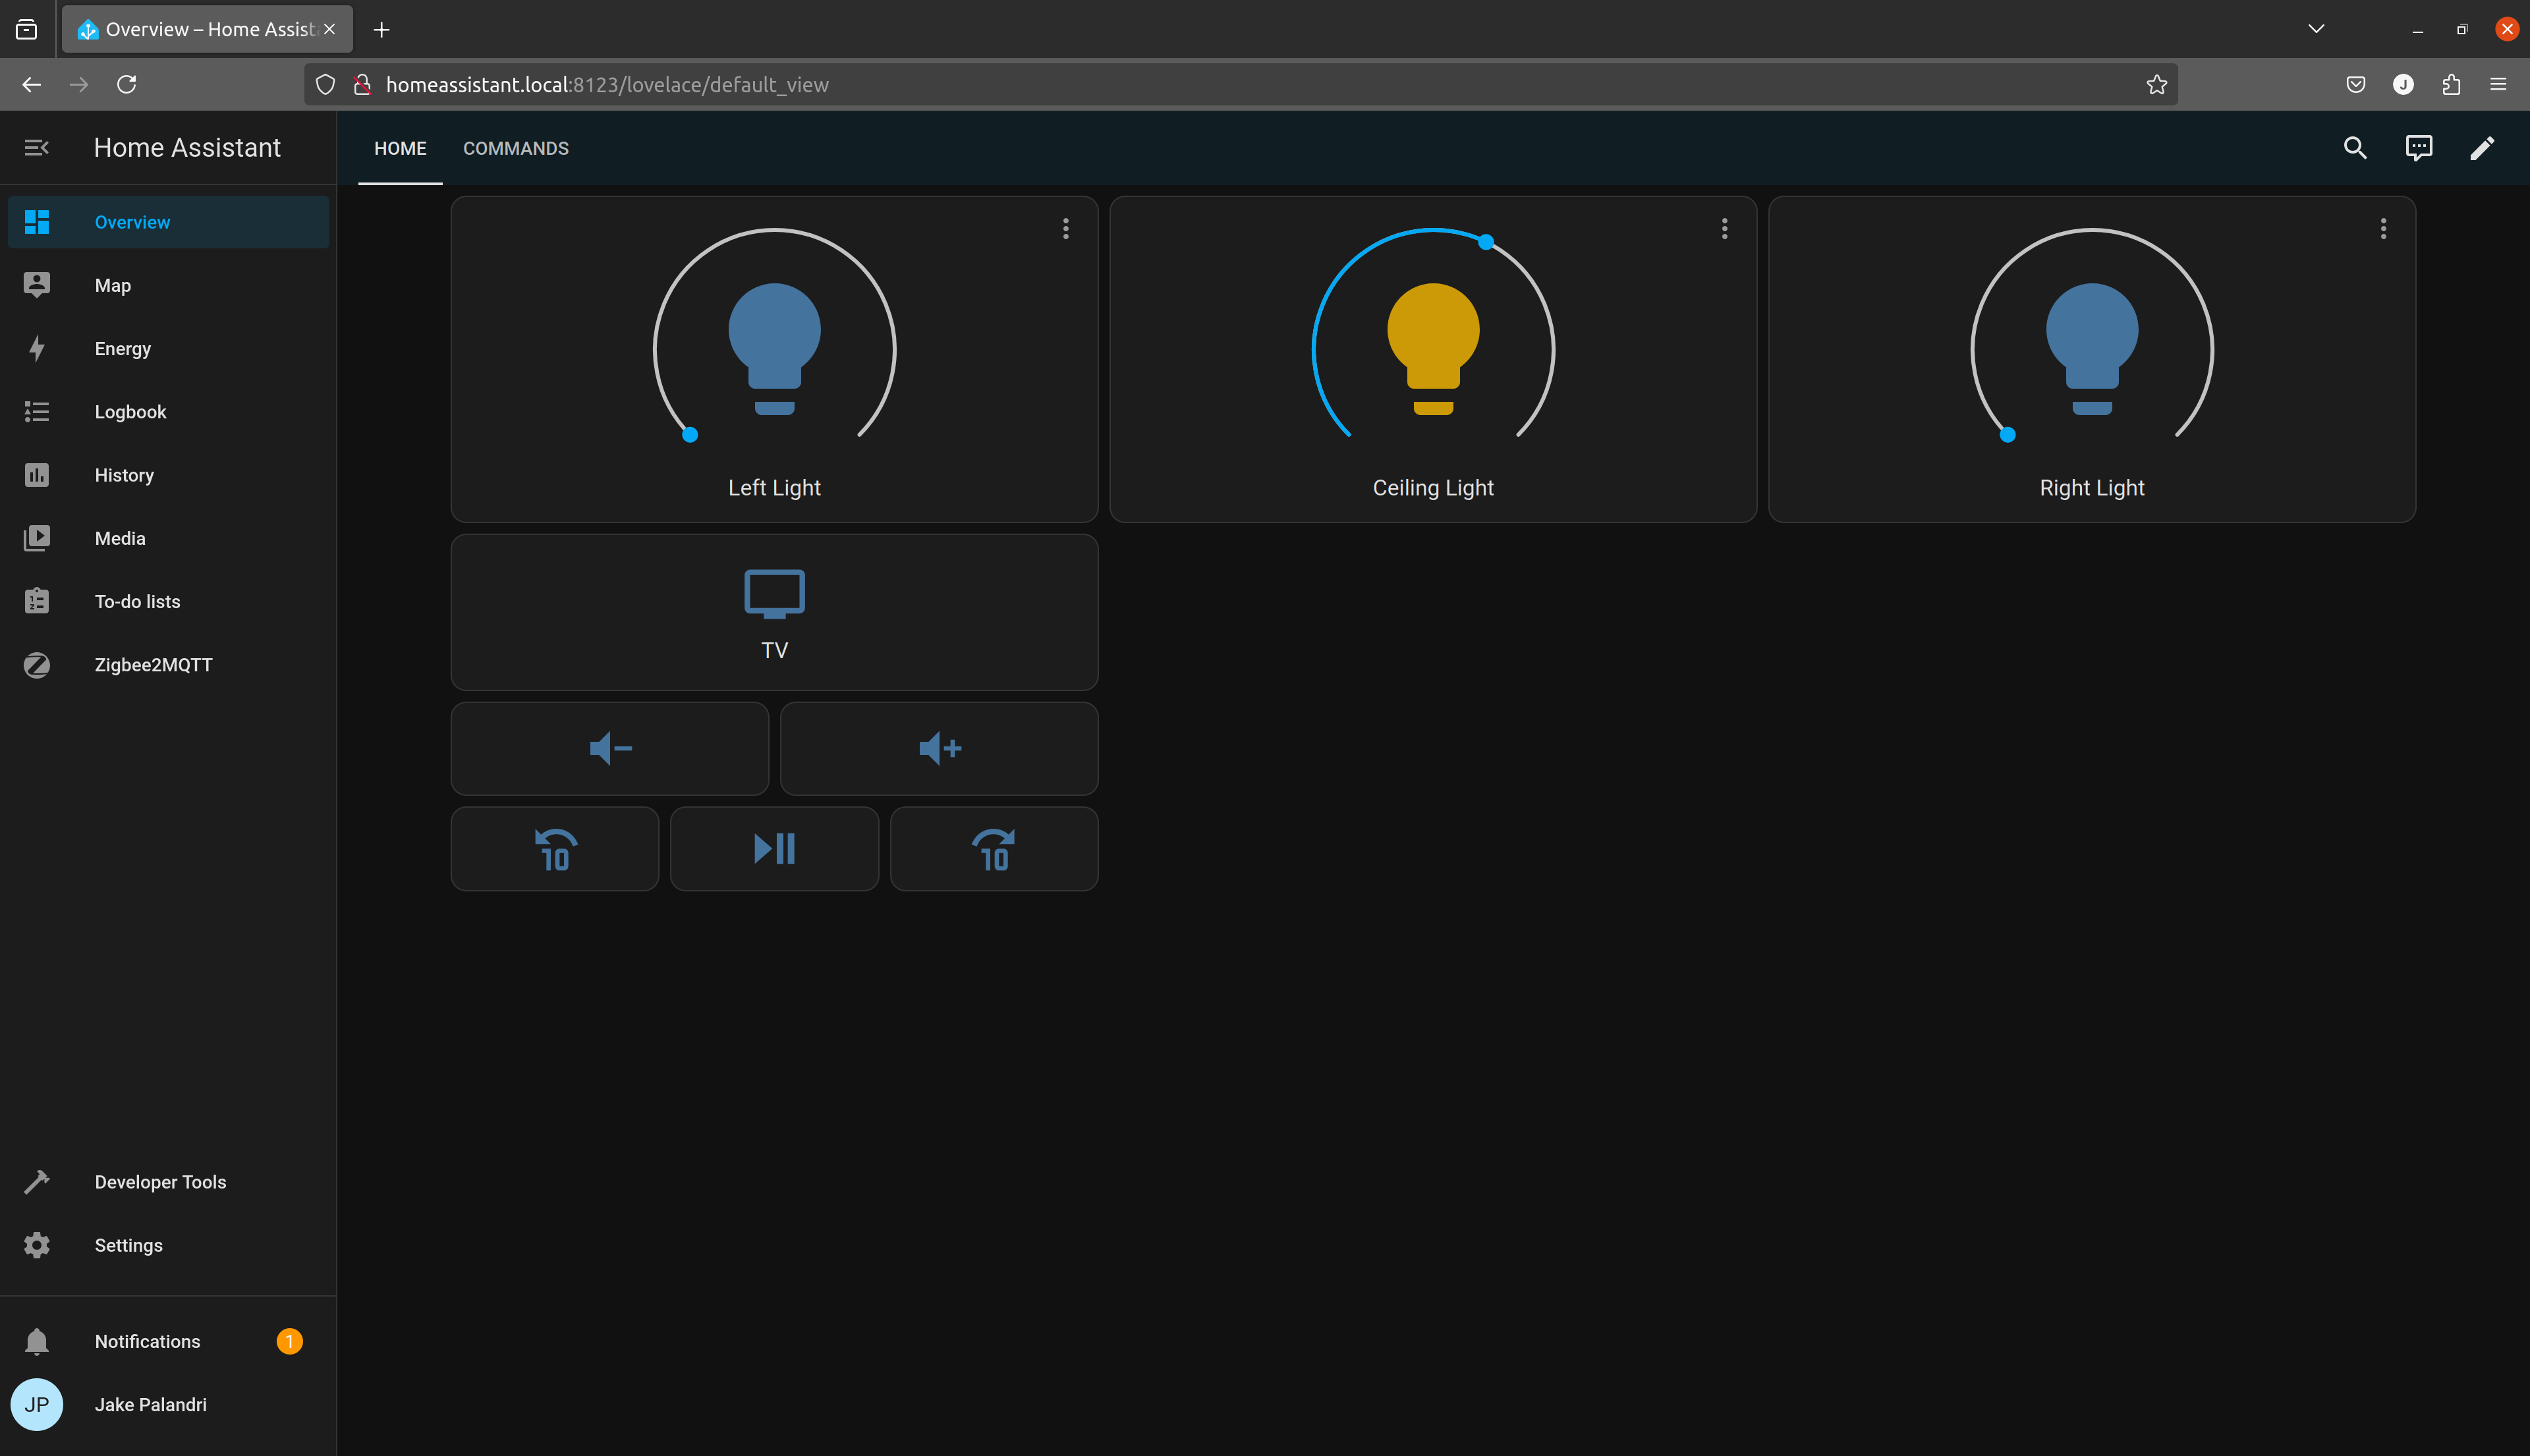
\includegraphics[width=0.9\pdfpagewidth]{Home Assistant.png}}
    \label{fig:home_assistant}
\end{figure}

The Sonoff Zigbee dongle, which is attached to the Raspberry Pi, along with the Ikea light bulbs and IR emitter were primarily chosen for their low price points.
Zigbee is an open source communication standards with lower fees for accreditation than other competing standards such as Z-Wave, therefore their products tend to be cheaper than their Z-Wave counterparts.
The dongle is required in order to communicate between Home Assistant and the smart devices.
The light bulbs and IR emitter were purely chosen as two examples to demonstrate the functionality of the system.
Any competing standard devices or different device types entirely would also be valid choices for the system depending on user needs.

The components should be set up as shown in Figure~\ref{fig:physical_setup_diagram}.

\begin{figure}[H]
    \caption{Physical Setup Diagram}
    \makebox[\textwidth][c]{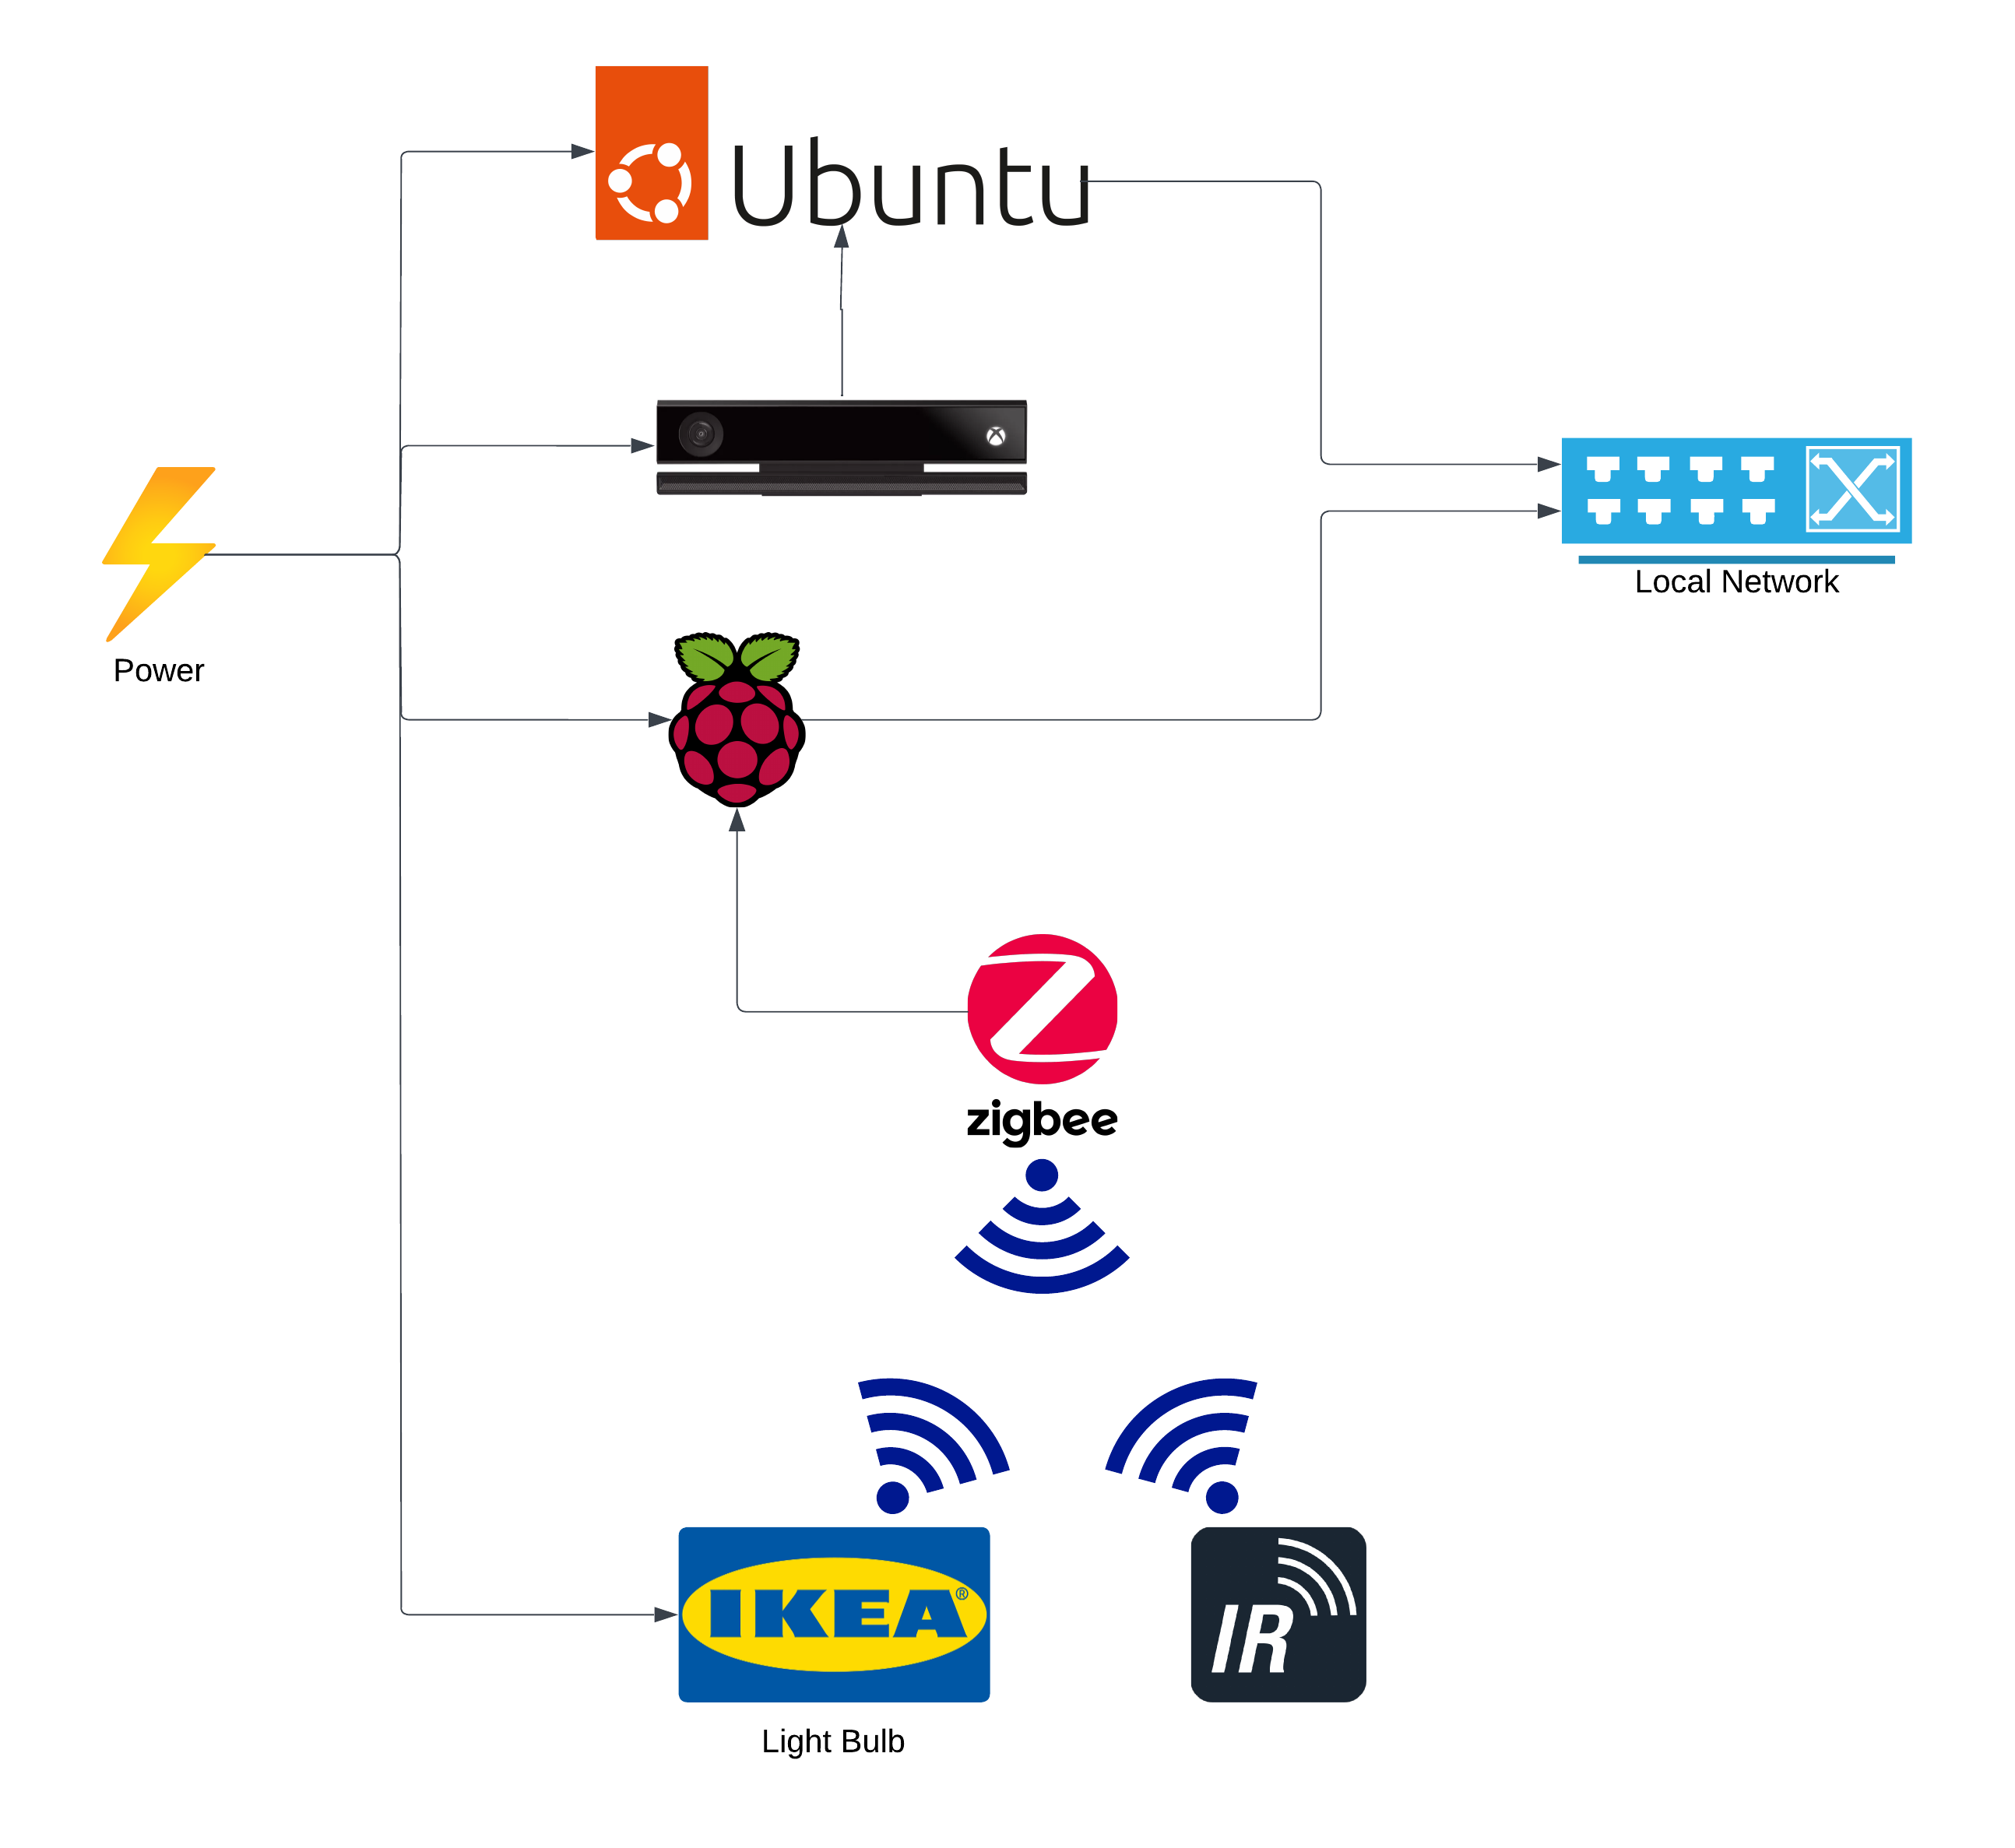
\includegraphics[height=0.6\textheight,angle=0]{Physical Setup Diagram.png}}
    \label{fig:physical_setup_diagram}
\end{figure}

\section{Software Components}
The key software components used in the development of this system include the following:
\begin{itemize}
    \item ROS
    \item ROS Client Library for Python (rclpy)
    \item Home Assistant
    \item Messaging Queuing Telemetry Transport (MQTT)
    \item Vosk Speech Recognition
    \item YOLO
    \item Python Web server
    \item TypeScript frontend
\end{itemize}

The proposal to use ROS to control devices in the smart home was made very early in the research stages.
This was because many of the robots and devices existing in the lab already operated on ROS.
Building the smart home on the same system would allow for further research and development into getting these projects working cohesively with one-another, as there are some operations that can be performed by robots in the lab, such as pointing to and retrieving an item, that could be useful in a smart home.
In it's current state, the commands to the smart home are accessible by other devices on the ROS network, however there is no integration with the robotics work being done, but this does allow for future expansion of the project.

Rclpy is the ROS library for Python and was one of only two options for development.
The alternative was a C++ library, however, due to the nature of the project, utilising AI and the lack of C++ skills upon embarkment of the project, rclpy was chosen to write the code for custom ROS nodes.
This is where the gesture recognition software operates as well as the speech to text model and voice command recognition nodes.

Home Assistant was chosen because, as an open source home automation platform, it allows users to customise their environment to their liking to a much higher degree than other mainstream platforms such as Apple HomeKit or Google Home.
This allowed a simple integration with the ROS components of our system as there was much more choice for methods to communicate between the platforms, nothing was locked down.

MQTT is a lightweight publisher/subscriber machine to machine messaging service.
This, together with zigbee2mqtt, allows the ROS nodes to send an MQTT message over the network and control Zigbee devices in Home Assistant directly.
This was selected due to its lightweight messaging service, cheaper products and simplistic implementation.
It is worth noting that using MQTT does not limit users to using Zigbee devices as the MQTT messages can be used to trigger automations in Home Assistant.
If a user determines that bluetooth, Wi-Fi or Z-Wave devices are more suitable for their requirements, then they are still able with no extra work required.

Vosk's speech-to-text (STT) models were selected for two main reasons.
Firstly, these are the same models used by other robots in the Human Robot Interaction lab where this system was deployed.
Maintaining a smaller number of tools makes the environment far easier to manage as functionality expands.
Additionally, Vosk supports streaming audio directly from a microphone to the model, whereas many other local STT models only support processing entire audio files.
Other models such as OpenAI's local Whisper models were tested in development, however the inability to stream audio made reliably interpreting the audio challenging.
YOLO was also selected as this was already in use by other systems in the lab and it provides a skeletonisation feature which allows the extraction of the coordinates of key points on a users body to track their poses and gestures. 

Python and TypeScript were selected for their simplicity in development with TS chosen over JavaScript (JS) for it's strict typing and as an extension challenge for the developers, previously unexperienced with TS.
Other languages for the backend web server and the frontend web app are also suitable choices.

\section{Component Interactions}

The process of enabling communication between ROS 2 and the Kinect camera took many iterations of testing throughout Thesis A, and resulted in a somewhat convoluted setup as shown in Figure~\ref{fig:kinect_ros}.
However, this was necessary for the goals of this thesis.
The Institute of Artificial Intelligence at the University of Bremen (IAI) has developed a set of drivers to allow communication between the Kinect and ROS 1, and another user created a fork of this repository to support OpenCV 4.0, an open source CV library, which was required for this deployment.
Since there is no existing Kinect bridge for ROS 2, the data from the Kinect must be processed first by ROS 1 and passed through to ROS 2. Because of this, the operating system required is Ubuntu 20.04, Focal Fossa, as this Linux distribution (distro) supports multiple versions of both ROS 1 and ROS 2, allowing communication between one another.
OpenKinect's Libfreenect2 drivers are required in order for IAI's Kinect 2 Bridge to access the data from the sensors on Ubuntu.
Finally, Open Robotics, the developers of ROS, provide a bridge between ROS 1 and ROS 2 that allows the translation of the topics, services, and actions between nodes in either direction.
These tools, in conjuction with ROS 1 distro Noetic Ninjemys, and ROS 2 distro Foxy Fitzoy, ROS 2 is able to access the data from the Kinect.

\begin{figure}[!htb]
    \caption{Kinect to ROS 2 Layers}
    \makebox[\textwidth][c]{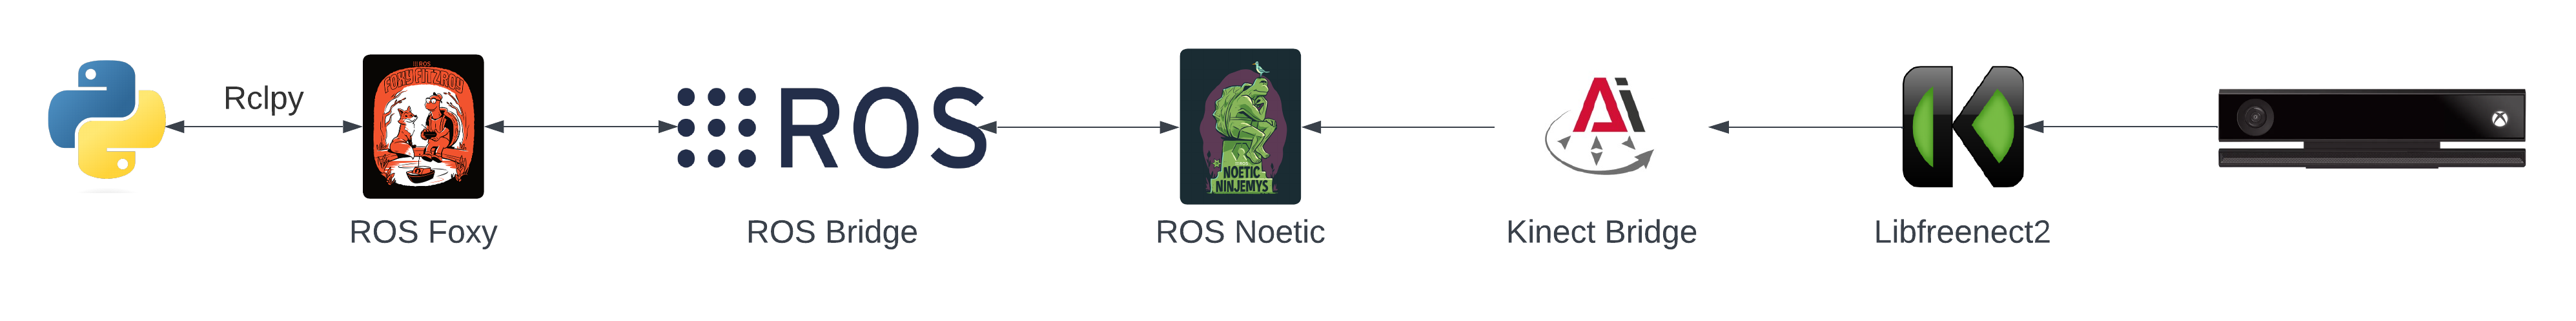
\includegraphics[width=0.9\pdfpagewidth]{ROS Kinect Layers.png}}
    \label{fig:kinect_ros}
\end{figure}

To integrate this with the current system, rclpy is used to process and register the gestures from the users and signals are then sent to the Home Assistant server on the network via MQTT.
A Raspberry Pi 3, is used to run the Home Assistant server along with an MQTT broker, and zigbee2mqtt, a service to bridge mqtt signals directly to zigbee smart devices.
From there, Home Assistant is able to control the smart devices over the zigbee network through manual control from the user or automations.

Using rclpy, there are two ROS nodes created to process the speech and the user's gestures.
The STT node takes audio directly from the computer's built-in microphone and streams it to Vosk to process the speech.
The result of the Vosk model is then published to a topic on the ROS network.
The second node subscribes to both the STT topic published by the first node, and the topics created by the Kinect sensors through the layers of translation from the camera to ROS 2.
This then processes the voice commands at the same time as the gestures and will send the MQTT message to trigger devices.

Finally, there is a web app that allows users to customise which voice commands are available to control their devices.
This is available on the network through a local IP address, or within Home Assistant as shown in Figure~\ref{fig:command_interface}.
The web app accesses a JavaScript Object Notation (JSON) file on the system that contains all device types available in the home and their associated commands.
From here the user can add, modify or remove commands and device types entirely depending on the needs of their home.
This modifies the JSON file on the system, which in turn triggers an update in the ROS node to ensure that only valid commands are being checked for.

\begin{figure}[!htb]
    \caption{Command Web Interface}
    \makebox[\textwidth][c]{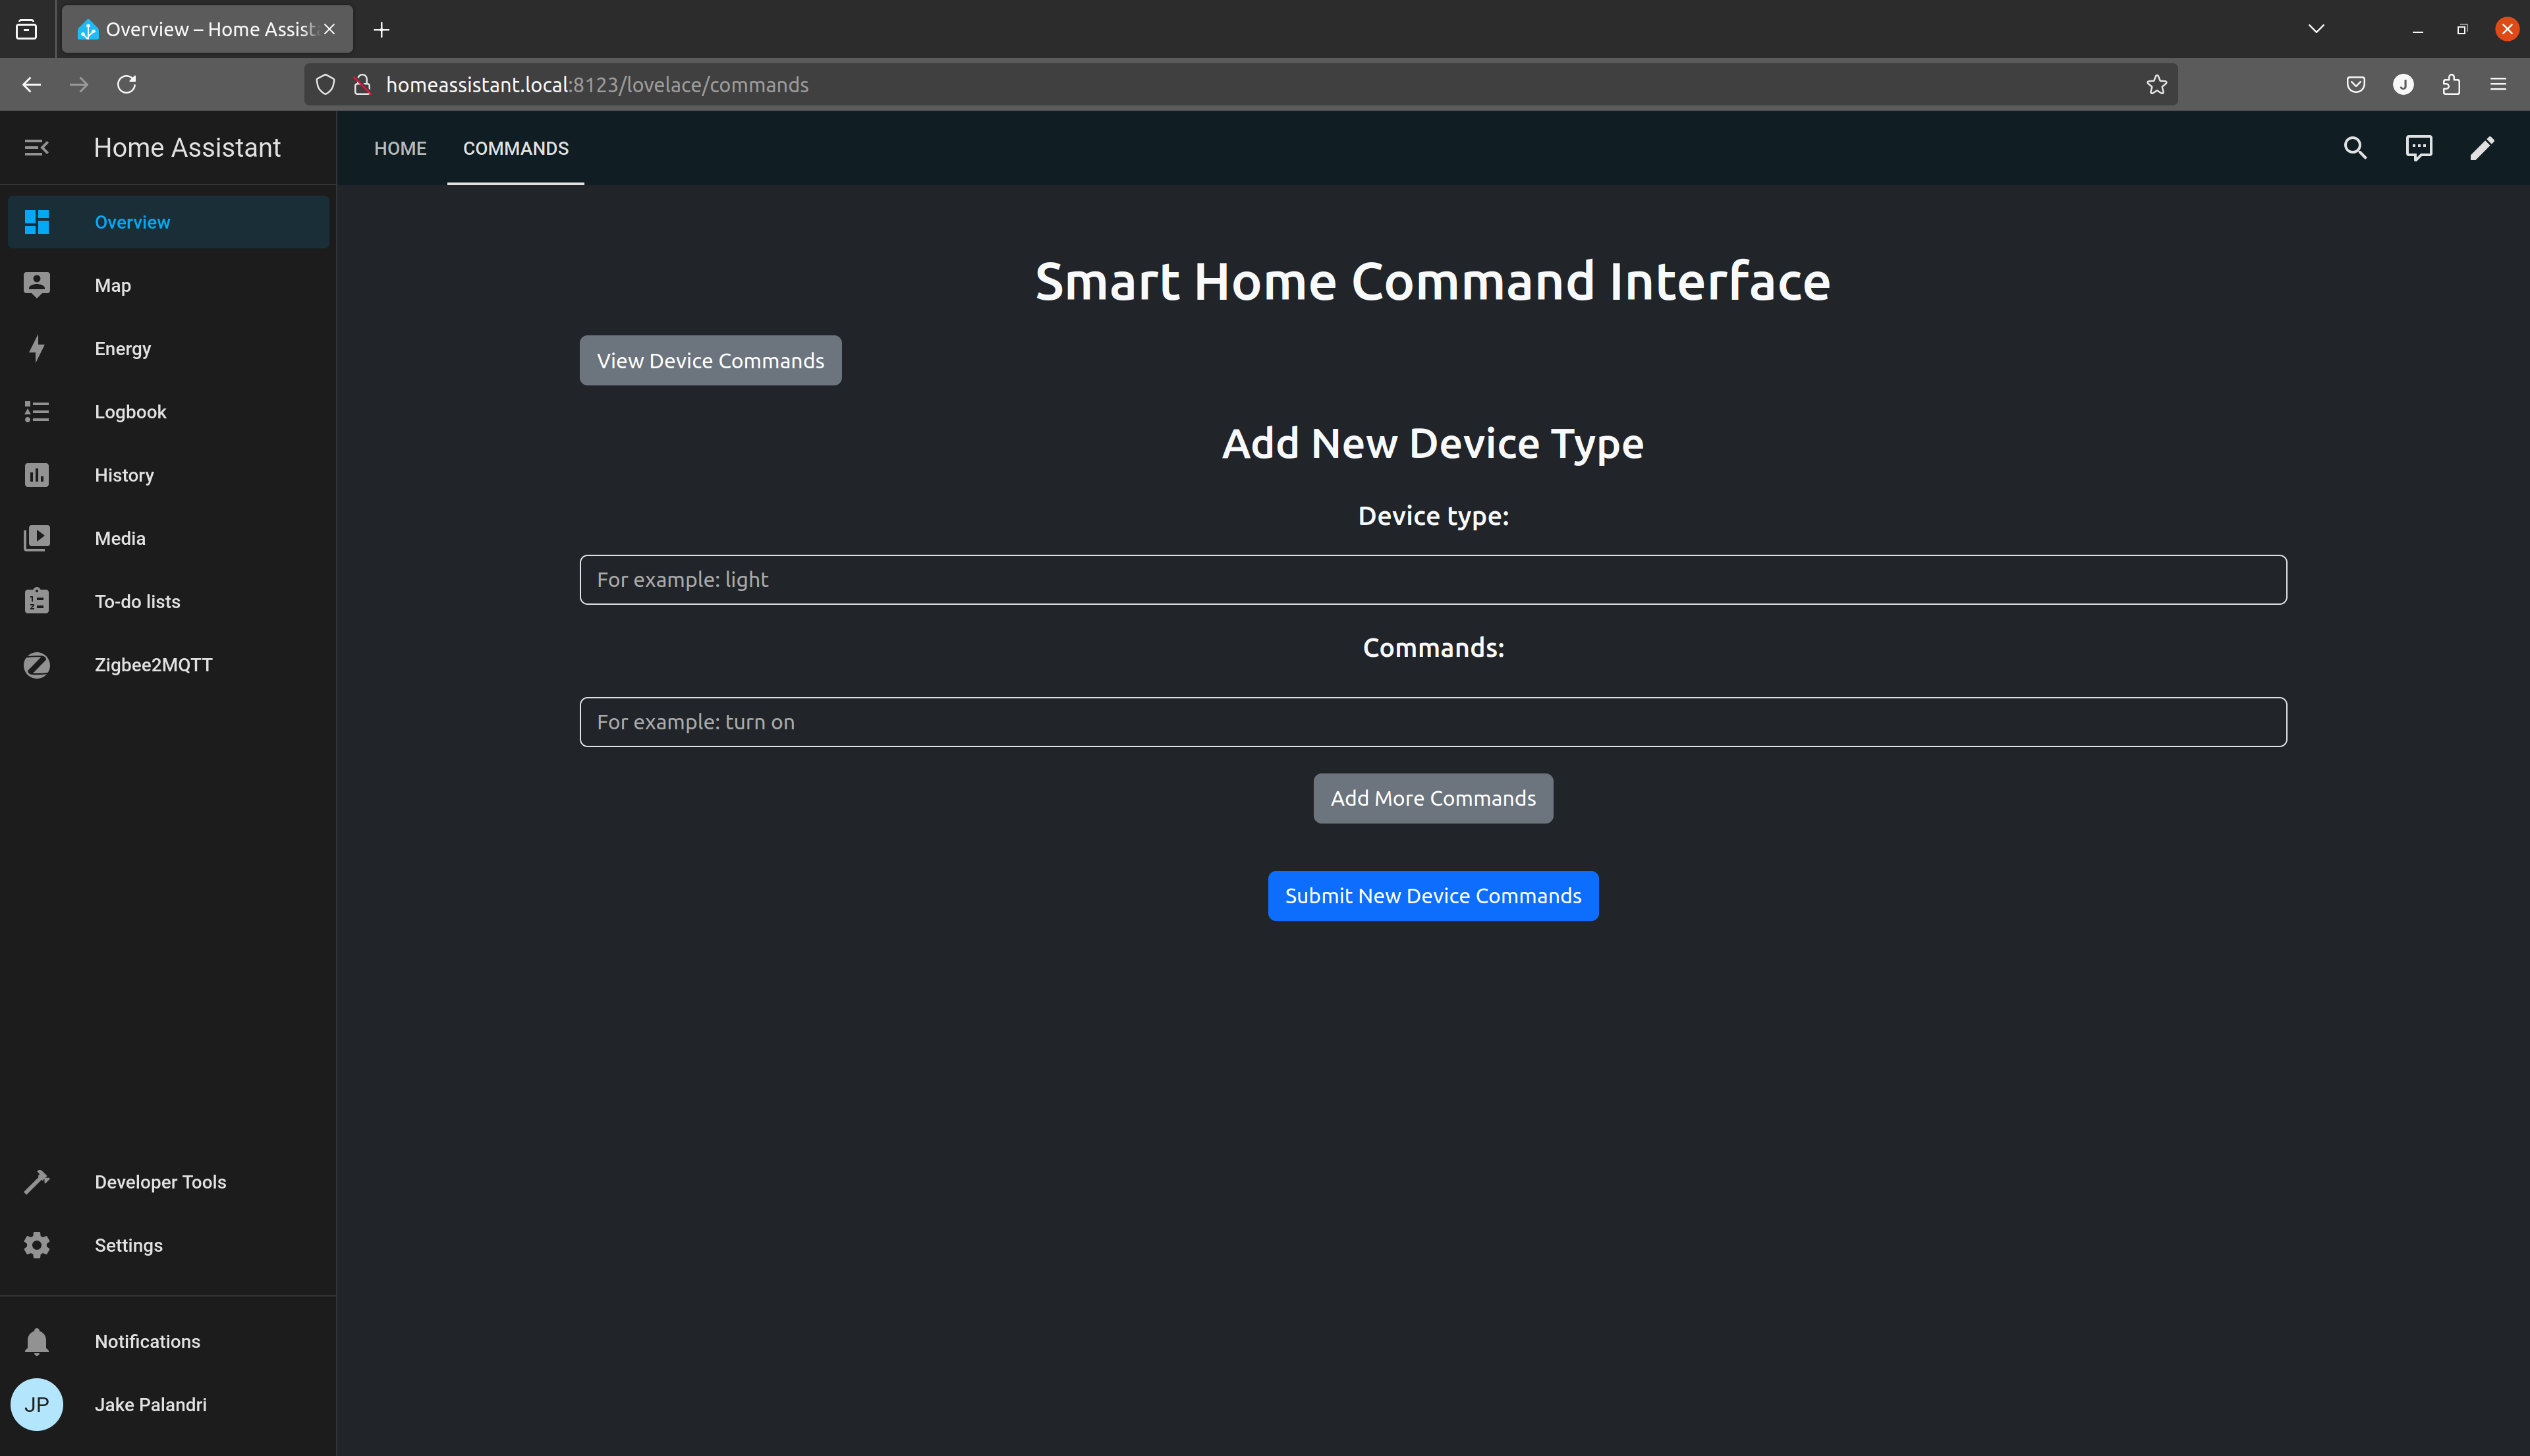
\includegraphics[width=0.9\pdfpagewidth]{Command Web Interface.png}}
    \label{fig:command_interface}
\end{figure}

\section{Code Logic}

Once the Kinect data and STT result has reached the final ROS node, there are primarily two processes running concurrently in order to trigger device commands.

First, with each frame from the Kinect's camera, the image callback is triggered which determines a users gesture and then stores it for use later by the voice commands process.
To determine a user's gesture, eight points on the users body are extracted using YOLOv8.
The hip, shoulder, elbow and wrist of both the left and right sides.
Then, using the depth data from the Kinect, the pixel coordinates from the image can be converted to 3-Dimensional world coordinates.
In case of any errors in YOLO selecting a point just outside the users silhouette, the depth value is taken as the point closest to the camera within a five pixel radius of the point.
Using the wrist and elbow coordinates, a vector can be created to determine which direction a user is pointing.
This is done by extending this vector and intersecting it with the bounding box that is the dimensions of the room.
Then it can be determined which wall, floor or ceiling is being pointed at.
A gesture is only registered if the distance from the users wrist to their hip or their shoulder surpasses a pre-defined threshold.
The gesture is then stored in a list as a history with an associated timestamp with a gesture being stored at 250 milliseconds intervals and storing the last 10 seconds of gestures.

At the same time, whenever the STT node sends a new string the speech processing callback is triggered.
The output from Vosk provides multiple possibile interpretations of the speech in order to minimise misinterpretations.
Each of these alternatives is checked to see if the sentence begins with the chosen wake word, set to ``home'' by default.
The wake word is not required to trigger a command but is required for the user to receive feedback for an invalid command.
This was done so that if a user forgets to use the wake word then if a valid command is given then it will still trigger a result.
However, if regular speech is picked up not intended to control a device, then the invalid command feedback is not triggered.

Following this, each of the alternative interpretations from Vosk are checked against the JSON object containing all the valid device types and commands.
These are checked against a regex string in order to allow users to speak in a more natural manner and still trigger the correct device with other superfluous words in the command.

The regex string for matching a command for a single device is:
\begin{center}
    \texttt{rf".*\textbackslash b\{command\}\textbackslash b.*\textbackslash bthat\textbackslash b.*\textbackslash b\{device\}\textbackslash b.*"}
\end{center}
For the case where the command is ``turn on'' and the device is a ``light,'' this gives users the ability to say the simple command ``turn on that light'', or speak more naturally and say ``could you turn on that light over there for me please.''

The regex string for matching a command for a all devices of a single type is:
\begin{center}
    \texttt{rf".*\textbackslash b\{command\}\textbackslash b.*\textbackslash b(all|every)\textbackslash b.*\textbackslash b\{device\}s?\textbackslash b.*"}
\end{center}
This gives users the option to say the commands ``turn on all lights,'' or ``turn on every light,'' or more naturally ``can you turn on all of the lights please.''

Once a command is matched, it is added to a list, and once each of the device types and commands is checked against the command with the latest match is selected.
This is done so that a user can correct themselves mid-sentence and still trigger their intended command.
For example, a user might say ``can you turn on that light, I mean that fan.''
This would trigger the automation to turn on the fan.
Once a command is recognised, the timestamp at which the word ``that'' is said is compared to the history of gestures and the gesture with the closest timestamp to the keyword is selected.

If no match is found for a given alternative interpretation from Vosk, the process loops.
If no match is found at all, and a wake word was supplied, then an audio cue is triggered to let the user know that their command was not recognised and to try again.
Additionally, if the user gives a valid command but does not gesture to point to their device, another audio message is relayed to the user to ask them to gesture when giving commands.
Finally, if a match is found, the command message is sent over MQTT and captured on Home Assistant to trigger custom automations set up by the user.